\chapter{Data Selection}
\label{cha:data_selection}

\section{Structure of data and data exploration}
\label{sec:data_exploration}
The selected dataset onto which a classification model shall be learned is provided by Kaggle\footnote{2017 Kaggle Inc}. It is named \textit{The movies Dataset}\footnote{Link to the dataset: \hyperref[https://www.kaggle.com/rounakbanik/the-movies-dataset]{https://www.kaggle.com/rounakbanik/the-movies-dataset}} and contains metadata of approximately 45,000 movies in its raw format. It is provided and updated by Rounik Banik. The complete dataset consists out of several files in\textit{csv}-format containing data about movie casts, metadata and external scores. The main file used during preprocessing is named \textit{movies-metadata.csv}. This csv-file contains 24 columns in total, which can be seen in the graphic below.
\begin{figure}[ht]
	\centering
		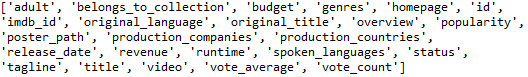
\includegraphics[width=\textwidth]{images/Raw_dataset_headers.png}
	\caption{Columns of the file \textit{movies-metadata.csv}}
\end{figure}

%Due to the multitude of attributes, it is essential to extract the relevant values for the implementation of a well-functioning classifier. Many values have no effect on the financial success of a movie and can therefore be ignored. This includes, for example, the columns...

The structure of the individual features is very different. In addition to boolean values, strings and numeric float values (e.g \textit{budget} or \textit{runtime}), many attributes contain longer texts (e.g \textit{overview}), arrays or even a list of JSON objects (e.g.\textit{production-countries}). These different formats must be taken into account in the preprocessing and need to be processed and extracted individually.
\\\\
%\section{Basic data exploration}
Exploring the dataset it can be noticed that the overall quality varies significantly. This can be attributed to the fact that it is maintained by a community and is not provided by a larger organization or company. Therefore, a demanding quality assurance process is difficult to realize. An important aspect of the quality of a dataset is that it contains values for the majority of its records. The examined dataset has a high amount of records containing missing values. This is especially true for older movies (before 1960), which contain only few information. Critical for this project is the presence of values of the attributes \textit{revenue} and \textit{budget}, which are used to determine the financial success of the movie. Here around 34,000 records are containing zero or missing values in either the revenue or the budget column.

In addition to that, there is no indication about the currencies of numerical financial attributes and a lot of values are inconsistent in respect to scaling. For example a movie having an actual revenue of \$ 312 MM and a budget of \$ 240 MM is given with a \textit{revenue} value of \textit{240,000,000} as a float number whereas the \textit{budget} value contains the float number \textit{312}. For the successful outcome of this project it is critical to keep those aspects in mind for later preprocessing steps, otherwise the result will be distorted.

Speaking of those issues it is also worth mentioning that the chosen dataset contains movie metadata from the past 60 years. With respect to today's economics a lot of things changed in movie production and consumption. Aspects that have influenced movie economics are for example price structures, inflation and globalization. But also consumer behavior changed drastically. Therefore it was decided to introduce a new attribute to the dataset, which will be called \textit{productivity}. This value describes the ratio of the revenue and the budget of the movie and expresses the success of a movie in this project. A \textit{productivity} of $1.0$ implies that the investment to produce this movie was covered anything above $1.0$ is assumed as profit.
\\

To get a better understanding of the data and its relations a few examinations where taken and are presented in the table below.
\begin{center}
	\begin{tabular}{| l | l |}
	\hline
	Average budget & \$ 31.662.585 \\ \hline
	Average revenue & \$ 92.059.210 \\ \hline
	Average productivity rate & 2.8 \\ \hline
	3 Most common genres & Drama, Comedy, Thriller \\ \hline
	Average runtime & 94 min \\ \hline
	\end{tabular}
\end{center} 